\documentclass[11pt, a4paper]{article}

\usepackage{graphicx}
\usepackage[a4paper,top=3cm,bottom=2cm,left=2cm,right=2cm,marginparwidth=1.75cm]{geometry}
\usepackage[english]{babel}
\usepackage[utf8x]{inputenc}
\usepackage{subfig}
\usepackage{float}
\usepackage{amsmath}
\usepackage{amssymb}
\usepackage{mhchem}
\usepackage{hyperref}
\usepackage{tikz}
\usepackage{cancel}
\usepackage{bm}

\graphicspath{ {./images} }
\newcommand*{\qed}{\hfill\ensuremath{\quad\square}}%
\newcommand*{\rad}{\ensuremath{\,\text{rad}}}
\newcommand*{\R}{\ensuremath{\mathbb{R}}}
\newcommand*{\C}{\ensuremath{\mathbb{C}}}
\renewcommand*{\Re}{\operatorname{Re}}
\renewcommand*{\Im}{\operatorname{Im}}
\renewcommand*{\epsilon}{\varepsilon}
\renewcommand*{\phi}{\varphi}
\renewcommand*{\d}{\text{d}}

\DeclareRobustCommand{\uvec}[1]{{%
  \ifcat\relax\noexpand#1%
    % it should be a Greek letter
    \bm{\hat{#1}}%
  \else
    \ifcsname uvec#1\endcsname
      \csname uvec#1\endcsname
    \else
      \bm{\hat{\mathbf{#1}}}%
     \fi
   \fi
}}

\makeatletter
\renewcommand*\env@matrix[1][*\c@MaxMatrixCols c]{%
  \hskip -\arraycolsep
  \let\@ifnextchar\new@ifnextchar
  \array{#1}}
\makeatother

\newtheorem{theorem}{Theorem}
\numberwithin{equation}{section}
\numberwithin{figure}{section}

%------------------------------------------------
%Templates for images and figures
% \begin{figure}[h]
%   \centering
%   \subfloat[caption 1]{{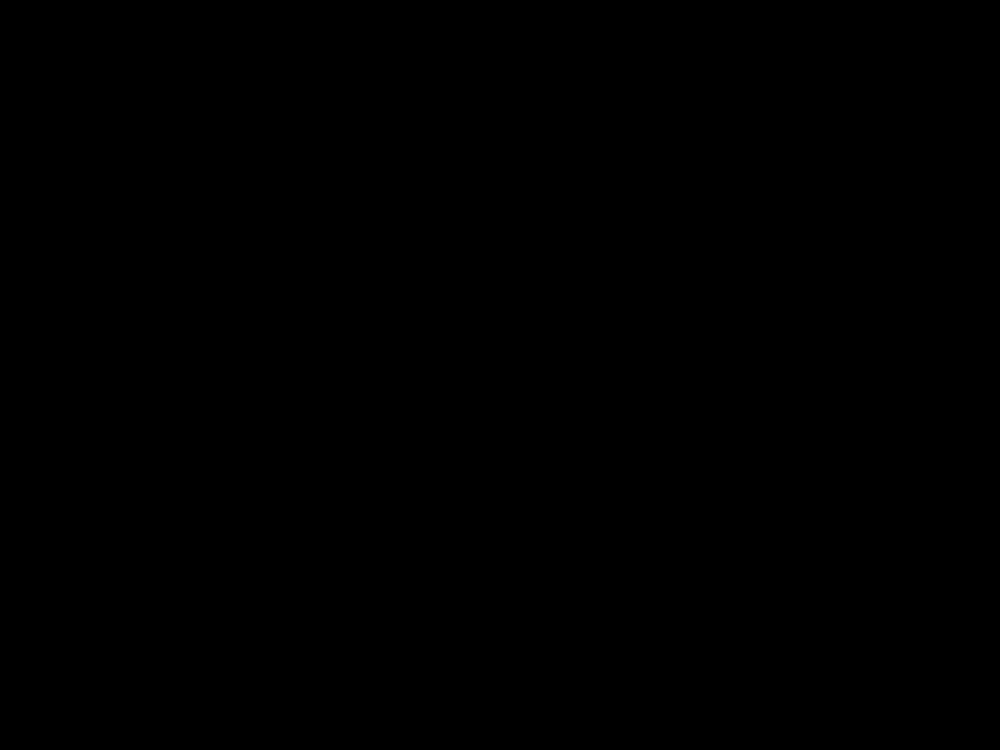
\includegraphics[width=30mm]{images/placeholder.png}}}%
%   \qquad
%   \subfloat[caption 2]{{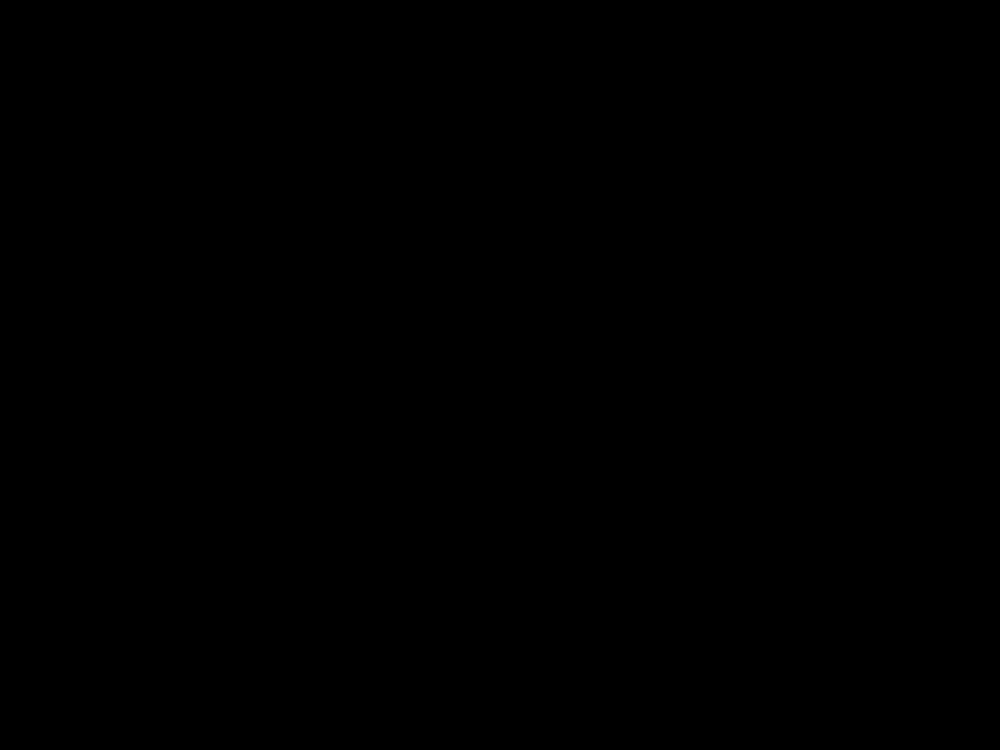
\includegraphics[width=30mm]{images/placeholder.png}}}%
%   \caption{Description}
% \end{figure}

% \begin{figure}[h]
%   \centerline{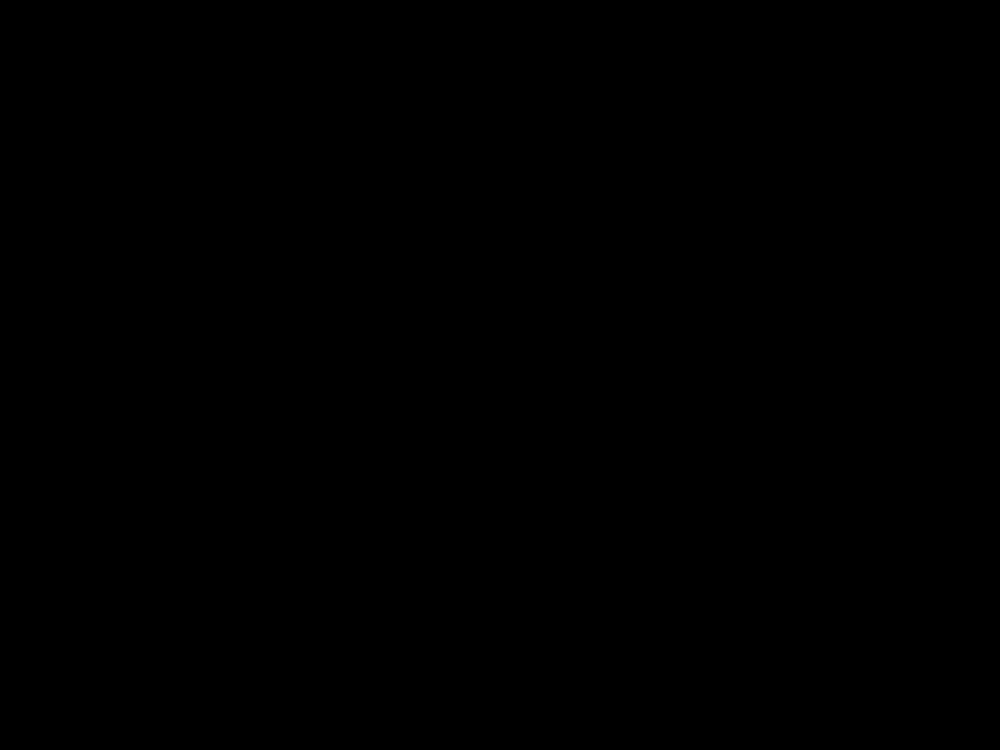
\includegraphics[width=50mm]{images/placeholder.png}}
%   \caption{Description}
% \end{figure}

%Template for a simple table 
%\begin{table}[h]
%   \caption{Description} %title of the table
%   \centering % centering table
%   \begin{tabular}{l rr} % creating three columns
%     \hline\hline %inserting double-line
%     & & \\ [0.5ex] % Insert half line vertical spacing
%     \hline % inserts single-line
%     & & \\ 
%     & & \\
%     & & \\
%     & & \\
%   \hline % inserts single-line
%   \end{tabular}
%   \label{tab:hresult}
% \end{table}
%-----------------------------------------------

\begin{document}
\setcounter{section}{2}
\section{Newton-Euler equations}

\subsection{Linear momentum}
\subsubsection{Single particle systems}
The definition of linear momentum is given as:
\begin{equation}
  \vec{p} = m\vec{r}
\end{equation}
When we recall Newton's original formulation for the second law we find that:
\begin{equation}
  \Sigma \vec{F} = \frac{\d(m\vec{v})}{\d t} = m\vec{\ddot{r}} = \vec{\dot{p}}
\end{equation}
Thus the sum of all forces in a system is nothing but the rate of chage of momentum with respect to time. We can integrate $\Sigma \vec{F}$ with respect to time to find that:
\begin{equation}
  \int_{t_0}^{t_1} \Sigma \vec{F}\,\d t = \vec{p}(t_1) - \vec{p}(t_0)
\end{equation}
Which is nothing but the change in momentum over some time interval $[t_0, t_1]$. This quantity is referred to as impulse.

\subsubsection{Multi-particle systems}
We can extend the definition of equation 3.1 to any systen of $N$ particles. We do this by adding up all the internal and external forces acting on a particle together:
\begin{equation}
  \label{eq:1}
  \sum_{i=1}^N (\vec{F}_i + \sum_{j=1}^N \vec{f}_{ij}) = \sum_{i=1}^N \vec{\dot{p}}_i
\end{equation}
Since we know all internal forces of a system should cancel out as they can't cause a net change in momentum of the system we get:
\begin{equation}
  \sum_{i=1}^N \vec{F}_i = \sum_{i=1}^N \vec{\dot{p}}_i
\end{equation}
We can simplify this even further. Recall the definition of the center of mass:
\begin{equation}
  \vec{r}_C = \frac{\sum_{i=1}^N m_i \vec{r}_i}{\sum_{i=1}^N m_i} = \frac{\sum_{i=1}^N m_i \vec{r}_i}{m}
\end{equation}
Taking the time derrivative of this we find that:
\begin{equation}
  \vec{\ddot{r}}_C = \frac{\sum_{i=1}^N m_i \vec{\ddot{r}}_i}{m}
\end{equation}
Which gives the following result when subsituting it back in equation \ref{eq:1}:
\begin{equation}
  \Sigma \vec{F} = m \vec{\ddot{r}}_C
\end{equation}
Thus the system of multiple particles can be described as an eqquipolent system with all forces acting on the center of mass of the system $C$.


\subsection{Angular momentum}
\subsubsection{Single particle systems}
Euler's second law of motion states that the angular momentum about some point $O$ and it's tiem derrivative can be given as:
\begin{align}
  \vec{H}_O &= \vec{r} \times (m\vec{\dot{r}})\\
  \vec{\dot{H}}_O &= \vec{\dot{r}} \times (m\vec{\dot{r}}) + \vec{r} \times (m\vec{\ddot{r}})
\end{align}
The cross product of a vector with itself will always be $\vec{0}$, thus the time derrivative of angular momentum is given as:
\begin{equation}
  \vec{\dot{H}}_O = \vec{r} \times (m\vec{\ddot{r}}) = \vec{r} \times \vec{F} = \vec{M}_O
\end{equation}
Which is nothing but the resultant moment vector about point $O$.

\subsubsection{Multi-particle systems}
This defention to can be extended to a system of particles by, again, summing all the individual components together:
\begin{equation}
  \sum_{i=1}^N \vec{r}_i \times (\vec{F}_i + \sum_{j=1}^N \vec{f}_{ij}) = \sum_{i=1}^N ( \vec{r}_i \times \vec{F}_i ) + \sum_{i=1}^N \sum_{j=1}^N (\vec{r}_i \times \vec{f}_{ij}) 
\end{equation}
Since Newton's 3rd law states $F_{action} = -F_{reaction}$ for every internal force $\vec{f}_{ij}$ there is another internal force $\vec{f}_{ji}$ which has the same line of action but in the opposite direction. Because of this we find the relation:
\begin{equation}
  \vec{\rho}_i \times \vec{f}_{ij} = -\vec{\rho}_j \times \vec{f}_{ji}
\end{equation}
This means the sum of all moments as a result of internal forces will form a moment pair with opposite direction, effictively canceling them all out. This leaves us with:
\begin{equation}
  \vec{\dot{H}}_O = \sum_{i=1}^N (\vec{r}_i \times \vec{F}_i)
\end{equation}
\end{document}